% Moved from Section 7 of the long version (sections/s7_delayed.tex) to keep the article at standard length:
% the full former Section 7, input right after the \section line of Supplement S7.
% Text copied verbatim; only references are adapted (M- = main article; no prefix = Supplementary Material).
% The displayed law eq:comb-law stays in the article; here it is cited with the prefix M-.

\subsection{A delayed term that vanishes on the forced orbit: a case study}\label{supp:std-delayed-law}

Two questions remain for a design that rests on the free voltage: whether a control law can spend the authority on the deviation from the forced orbit alone, and how robust the free voltage and the basin are to errors in the model. The first is answered by a case study of a published delayed term, the second by a Monte Carlo study (Section~\ref{supp:std-delayed-robust}).

The DVF command of Eq.~\eqref{M-eq:dvf} is replaced by the command $u(t)$ of Eq.~\eqref{M-eq:comb-law}, clipped as before, $V=\sat_{\Vmax}(u)$, and studied with $k_d=0$ (DVF\,+\,D). In the Laplace domain $U(s)=-\bigl[s\,K(s)+k_d\,E(s)\bigr]X(s)$ with $K(s)=g_1+g_2E(s)$ and $E(s)=1-e^{-sT}$. The delayed terms vanish on every $T$-periodic motion, since $E(im\omega_T)=0$ at every tooth-passing harmonic, so the forced orbit, its command $b(t)=-g_1\dot x_p(t)$ and the free voltage $u_0$ depend on $g_1$ alone, while a deviation from the orbit meets the full law. Without loop delay $K$ is positive real and the loop passive like DVF \citep{elliott2001feedback}. The law is published: its non-invasiveness is that of Pyragas-type delayed feedback \citep{pyragas1992continuous}, applied to milling by \citet{vandewouw2015ifac} and \citet{vandijk2015ijrnc}; \citet{li2022ijamt} fed back $x(t)-x(t-T)$ to lower the actuator voltage, and delayed feedback has countered regeneration in turning \citep{mancisidor2019mechatronics} and milling \citep{du2022time,du2024ijms}. It is used here to test whether linear margin translates into tolerance of disturbances under a hard clip. The models, the certificate with the delayed terms and the robustness study are detailed in Sections~\ref{supp:mc}--\ref{supp:delayed-robust}.
% src: README §13.2; src/c4_comb.py (docstring, model), src/c4_robust.py (controller); tests/test_c4_comb.py (test_comb_terms_vanish_on_the_settled_cut); paper/notes/novelty.md §1.6

Both families were designed by the authority rule of Eq.~\eqref{M-eq:feas}: $g_1$ is the largest gain up to \SI{3000}{\volt\second\per\metre} whose steady forced command stays within \SI{9}{\volt} up to 0.9 times the design's own linear limit, so that in effect the same gain is compared with and without the delayed term. With $g_2=\SI{2000}{\volt\second\per\metre}$ the linear limit rises by a median factor of 1.78 (1.44--2.10) over the 251 speeds (Fig.~\ref{fig:dlim}a). Much of this rise, however, lies at depths that are not usable: the limit exceeds \SI{32}{\milli\metre}, twice the cutter diameter, at 222 of the 251 speeds, against 71 for DVF, and with the depth capped at \SI{32}{\milli\metre} the median gain falls to 1.31; the cutting tests of \citet{ozsoy2026robust} went up to \SI{10}{\milli\metre}.
% src: results/c4_limits.npz (feas_g1: max |g1 - g1_DVF| = 9.7 V s/m); results/c4_summary.json (limits.feasible: d2000 ratio_to_dvf median 1.78, range 1.44-2.10); verification/paper/revision_runs.json (stored.depth_2D: d2000_above_32mm 222, dvf_above_32mm 71 of 251; median_ratio 1.781, median_ratio_capped_32mm 1.309); verification/targets/experimental_points.csv (tested depths up to 10 mm)

The clipped entries tell a different story (Fig.~\ref{fig:dlim}b). Simulated at 25 speeds with the \SI{9}{\volt} clip, the face-entry limit rises with D by a median factor of 1.72, but the step-entry limit by only 1.03 (0.98--1.27): from \SI{2100}{\rpm} upwards D changes it by at most \SI{1.1}{\milli\metre}, as this limit is set by saturation during the entry, not by damping. The band in which the outcome depends on the entry therefore widens, from a median width of 7.6 to \SI{26}{\milli\metre}. At the same forced command, adding the term with its certificate-optimal $g_2$, which was \SI{500}{\volt\second\per\metre} at every point, to the $g_1$ of the certificate-optimal DVF design widens the simulated basin (worst-phase critical kick) by a median factor of only 1.14 over 22 depth--speed pairs, by about 2 where the DVF certificate almost vanishes, and by 0.96--1.16 below \SI{18}{\milli\metre}; the certified kicks lie below the simulated ones at all 89 points where a kick of up to \SI{3}{\metre\per\second} caused chatter. The term is also fragile: the phase of $E(i\omega)$ alternates between lead and lag between tooth-passing harmonics, and with assumed second modes at 400--\SI{800}{\hertz} the design with $g_2=2000$ tolerates a loop delay of \SI{100}{\micro\second} but not \SI{200}{\micro\second}, against 300 but not \SI{400}{\micro\second} for DVF; a delay \SI{2}{\percent} longer than $T$ makes the term act on the forced orbit and lowers its linear limit to 0.87--0.93 of the nominal value, and with runout its worst command reaches \SI{9}{\volt} at 1.0--\SI{2.4}{\micro\metre}, against 1.1--\SI{4.5}{\micro\metre} for DVF.
% src: results/c4_entry.npz (face 1.45-2.12, median 1.72; step 0.98-1.27, median 1.03; from 2100 rpm +1.08 mm at most; band widths medians 7.56 and 25.88 mm); results/c4_summary.json (validate2: same_g1_over_dvf median 1.14 over 22 pairs; same_g1_near_dvf_limit 1.79-2.59, median 2.00; below 18 mm 0.96-1.16; all_cert_below_td 89/89); results/c4_summary.json (robust.by_rpm: loop delay 300/200/100/100 us for DVF/1000/2000/4000; runout_tolerance_um g2 = 2000 1.03-2.42, DVF 1.12-4.50; tau_us grid 0/50/100/200/300/400; c4_validate2.npz kind same_g1: g2 = 500 at all 25 points; tooth comb eps +2 %: limit 0.87-0.93); paper/figures/figure_numbers.json (fig10)

\begin{figure}[!tbp]
  \centering
  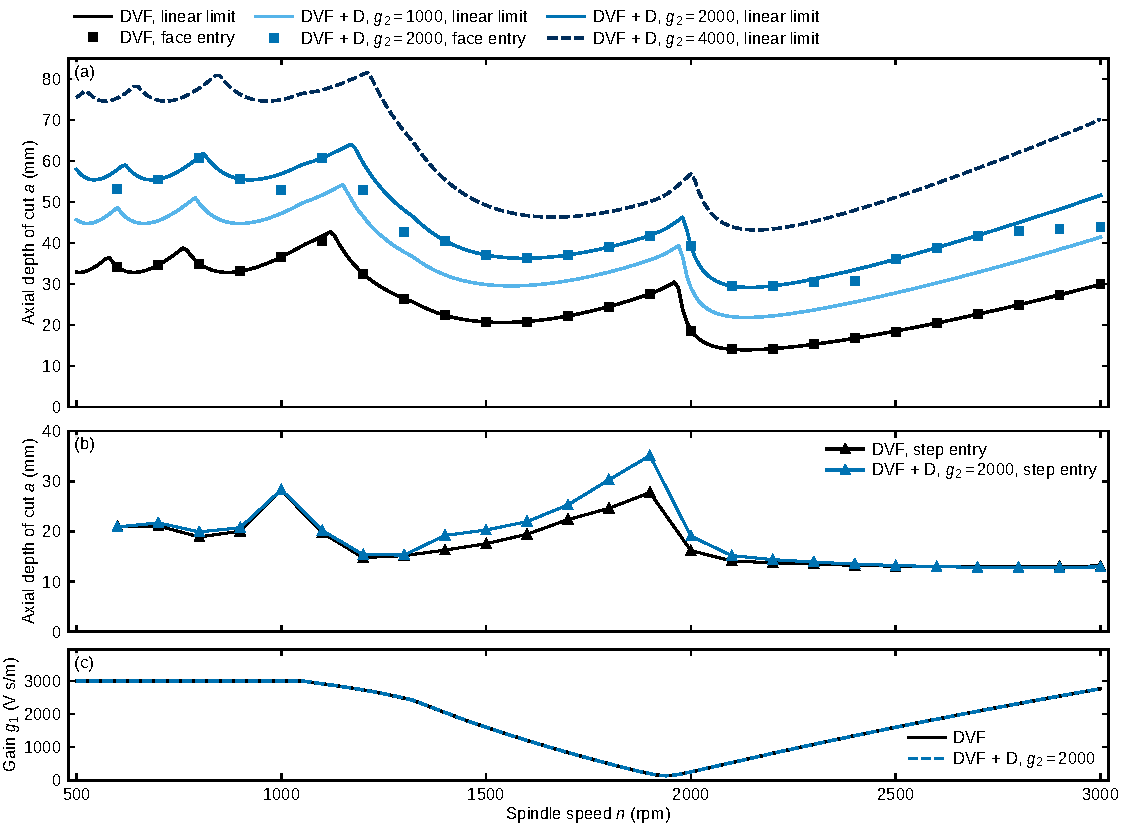
\includegraphics[width=0.86\textwidth]{figures/fig08_delayed_limits.pdf}
  \caption{The delayed term under the same authority rule ($g_1\le\SI{3000}{\volt\second\per\metre}$; steady forced command within \SI{9}{\volt} up to 0.9 of the design's own $\alim$). (a)~Linear limits of DVF and of DVF\,+\,D with $g_2=1000$, 2000 and \SI{4000}{\volt\second\per\metre}; squares: simulated face-entry limits ($\lvert V\rvert\le\SI{9}{\volt}$, 25 speeds) of DVF and of DVF\,+\,D with $g_2=2000$; dash-dotted: $2D=\SI{32}{\milli\metre}$, twice the cutter diameter. (b)~Simulated step-entry limits of the same two designs: the linear margin gained by the delayed term hardly reaches the clipped step entry.}
  \label{fig:dlim}
\end{figure}

The case study thus gives a negative result that matters for design: a law that raises the linear limit by 78\,\% and spends no authority on the forced orbit raises the depth reached by an abrupt entry by 3\,\%, because the entry transient, not the damping of the chatter mode, saturates the actuator. Linear margin is not tolerance of disturbances.

\subsection{Robustness of the residual authority and of the basin}\label{supp:std-delayed-robust}

The residual authority of the nominal design was sampled under errors in the model (Table~\ref{tab:mc}). The cutting coefficients were drawn independently and uniformly within $\pm\SI{10}{\percent}$ of their nominal values (in a second case $\pm\SI{20}{\percent}$), the natural frequency within $\pm\SI{5}{\percent}$, the damping ratio within $\pm\SI{20}{\percent}$, the actuator force constant within $\pm\SI{10}{\percent}$, the eccentric runout within 0--\SI{5}{\micro\metre}, the clip level within 8.1--\SI{9}{\volt} and the loop delay within 0--\SI{300}{\micro\second}; for 4000 samples per case the linear limit and the forced command, the worst over eight phases of the runout, of the $g=1500$ design were computed in closed form at depths fixed as fractions of the nominal $\alim$. At the design depth $0.9\,\alim$ the sampled cut is linearly unstable in 8--\SI{20}{\percent} of the samples, and its forced orbit reaches the clip in up to \SI{9}{\percent}; at $0.98\,\alim$ the two together take 32--\SI{79}{\percent}. Even at half the limit, the forced orbit reaches the clip in 69 and \SI{50}{\percent} of the samples at 2500 and \SI{2870}{\rpm}, where the nominal residual authority is only 1.5 and \SI{3.2}{\volt} at that depth. There the runout dominates (Spearman rank correlation with $u_0$ of $-0.62$ and $-0.83$), whereas near the limit the cutting coefficient, the natural frequency and the actuator constant dominate through the linear limit itself. Widening the range of the cutting coefficients to $\pm\SI{20}{\percent}$ raises the probability of linear instability at $0.9\,\alim$ to 15--\SI{22}{\percent}. In the simulator, with the sampled runout, clip and loop delay, the worst-phase critical kick at $0.9$ of the nominal $\alim$ was found for the first 25 samples at each speed (Section~\ref{supp:mc}). In one or two of them per speed the cut did not settle, being linearly unstable at the sampled parameters or, at \SI{2870}{\rpm}, its forced command exceeding the clip by several volts. In 92 of the other 93 samples the critical kick was 0.39--2.04 times its nominal value (medians 0.81--1.16 over the speeds) and below half of it in three, and in one no kick up to \SI{3}{\metre\per\second} ended in chatter. It followed the margin to the sampled linear limit (rank correlation 0.64--0.90) more closely than the residual authority (0.21--0.43), except at \SI{2870}{\rpm} (0.67 against 0.74), where the runout dominates the latter. Such samples show how the basin moves with the errors but bound nothing: with one or two unsettled samples in 25, the 95\,\% upper confidence bound on that probability is 18--\SI{23}{\percent}.
% src: verification/paper/mc_closed_form.json (levels.pm10/pm20.ranges; n_per_case 4000; speeds.*.fracs.*.p_unstable, p_saturated, u0_stable_median_V, dominant_u0_all, spearman_u0_all: 2500 rpm 0.5 runout -0.62, 2870 rpm 0.5 runout -0.83; nominal.u0_9V); mc_closed_form.py, mc_common.py (caches restored; nominal reproduces stored a_lim and bmax: checks.nominal)
% src (simulated): verification/paper/mc_kick.py/.json (protocol: first 25 samples of the pm10 draw, seed 20261124, 0.9 nominal a_lim, g 1500, phases 0/4/8/12 of 16, face entry, full memory, judged once per revolution); verification/paper/mc_kick_stats.py/.json (speeds.*: unsettled 2/2/1/2, unsettled_reasons linearly unstable at 1090/1420/2500, forced command at the clip at 2870; inf 1/0/0/0; finite 22/23/24/23; all.ratio_min 0.386, ratio_max 2.044, ratio_median_range 0.805-1.158; below_half_nominal 0/2/1/0; spearman_kick_vs_alim_margin 0.879/0.904/0.641/0.673; spearman_kick_vs_u0_worst_psi 0.209/0.416/0.432/0.735; cp95_upper_unsettled 0.231/0.231/0.176/0.231)

\begin{table}[!tbp]
  \centering
  \caption{Monte Carlo of the residual authority $u_0=V_{\mathrm{clip}}-\bmax$ of the $g=\SI{1500}{\volt\second\per\metre}$ design (closed-form zero-order model; forced command the worst over eight runout phases; 4000 samples per case; depth fixed at a fraction of the nominal $\alim$; parameter ranges in the text). $\pm\SI{10}{\percent}$, $\pm\SI{20}{\percent}$: range of the cutting coefficients. $u_0$ in volts; median over the linearly stable samples. Unstable: linearly unstable samples; clip: stable samples whose forced orbit reaches the clip ($u_0\le0$); both in per cent of the samples. These are frequencies over an assumed distribution, not a guarantee.}
  \label{tab:mc}
  \small
  \begin{tabular}{@{}rcccccrr@{}}
    \toprule
    Speed & $a/\alim$ & Nominal & \multicolumn{3}{c}{$\pm\SI{10}{\percent}$} & \multicolumn{2}{c}{$\pm\SI{20}{\percent}$}\\
    \cmidrule(lr){4-6}\cmidrule(l){7-8}
    (rpm) & & $u_0$ & median $u_0$ & unstable & clip & unstable & clip\\
    \midrule
    1090 & 0.5 & 4.72 & 3.69 & 0 & 0 & 0 & 0\\
     & 0.7 & 4.65 & 3.71 & $<1$ & 0 & 1 & 0\\
     & 0.9 & 4.69 & 3.96 & 20 & 0 & 20 & 0\\
     & 0.98 & 4.01 & 3.20 & 32 & 0 & 31 & 0\\
    \addlinespace
    1420 & 0.5 & 2.68 & 1.80 & 0 & $<1$ & 0 & 2\\
     & 0.7 & 8.72 & 7.79 & 0 & 0 & 0 & 0\\
     & 0.9 & 2.91 & 1.98 & 12 & $<1$ & 22 & 1\\
     & 0.98 & 1.79 & 1.21 & 48 & 2 & 49 & 2\\
    \addlinespace
    2500 & 0.5 & 1.49 & -0.65 & 0 & 69 & 0 & 65\\
     & 0.7 & 7.76 & 6.14 & 0 & 0 & $<1$ & 0\\
     & 0.9 & 2.79 & 1.58 & 11 & 4 & 15 & 8\\
     & 0.98 & 1.13 & -0.63 & 31 & 48 & 33 & 39\\
    \addlinespace
    2870 & 0.5 & 3.24 & 0.01 & 0 & 50 & 0 & 49\\
     & 0.7 & 5.99 & 2.29 & 0 & 19 & 0 & 19\\
     & 0.9 & 6.74 & 4.12 & 8 & 9 & 15 & 7\\
     & 0.98 & 5.04 & 3.30 & 34 & 3 & 39 & 2\\
    \bottomrule
  \end{tabular}
\end{table}
% src: verification/paper/mc_closed_form.json (nominal.<rpm>.u0_9V; levels.pm10/pm20.speeds.<rpm>.fracs.<frac>: u0_stable_median_V, p_unstable, p_saturated)

The clip level itself is a design choice (Section~\ref{supp:std-model-act}). Lowering it from 9 to \SI{8.1}{\volt}, which kept the peak actuator force at \SI{26.6}{\newton} in the deepest stable step entry at \SI{2500}{\rpm}, reduces the residual authority at $0.9\,\alim$ to 0.68--0.87 of its value and the worst-phase critical kick there to 0.76--0.88 of its value at the four speeds, close to the ratios of 0.78--0.89 that the describing function of Eq.~\eqref{M-eq:dfbasin} predicts; at \SI{2500}{\rpm} the forced command exceeds \SI{8.1}{\volt} already at 0.27--$0.46\,\alim$, by up to \SI{0.47}{\volt}, and again near $\alim$, so that with this clip the forced orbit itself is clipped there and the basin closes before the limit. A force limit enforced by lowering the clip is thus paid for in tolerated disturbance.
% src: verification/paper/protocol_clip_level.json (summary: ratio_of_minima 0.850/0.763/0.763/0.878 at 1090/1420/2500/2870 rpm, 0.9 a_lim, phases 0, 4, 8, 12; df_ratio_prediction 0.845/0.801/0.778/0.892; free_voltage_ratio_at_0p9alim 0.808/0.690/0.677/0.866; free_voltage_ratio_at_alim at 2500 rpm -0.038); verification/paper/support_runs.json (26.6 N at 8.1 V, deepest stable step entry at 2500 rpm, g = 1500); verification/paper/clip81_forced_command.py/.json (2500 rpm: intervals_above_clip_frac 0.27-0.46 and 0.9975-1, max_V 8.570 at 0.35 a_lim, V_at_a_lim 8.13; none at 1090, 1420, 2870 rpm)
